%O \textit{benchmark} Bench4Q define uma carga de trabalho, incluindo banco de dados, transações, regras de execução e de taxa de transferência e métricas de resposta.  Para expor a dinâmica de um sistema é necessário estimulá-lo através da carga de trabalho. Este componente é responsável por estimular o sistema através de cenários ou fenômenos \textit{burstiness}. Essa implementação é composta por classes e métodos, esse conjunto de código é um componente básico do \textit{benchmark} que refere-se a uma unidade de trabalho genérica que envia a carga para o sistema. O \textit{burstiness} inclue solicitações HTTP, chamadas de procedimento remoto, invocações de \textit{web services}, transações de banco de dados, comandos interativos ou também poderia ser composto de múltiplas tarefas de processamento, por exemplo sessões de cliente que compreendem várias solicitações ao sistema, etc \cite{Kounev2005}. Segundo \citeonline{Nobile2013} uma alteração na entrada (carga de trabalho) fará com que o sistema saia do estado de regime estacionário e entre em um período de regime transiente que descreve a dinâmica de um sistema, o regime transiente é calculado para uma entrada degrau unitário.

O objetivo deste trabalho é estender a carga de trabalho do \textit{benchmark} Bench4Q para que seja possível estimular o sistema a apresentar a sua dinâmica, e assim possibilitando a analise transiente do sistema, incorporando-se o modulo \textit{Demand} da arquitetura conceitual MEDC. 

Conforme apresentado no Capitulo \ref{chapter:revisao}, o \textit{benchmark} Bench4Q oferece uma interface gráfica para configuração e coleta dos dados, o que facilita a sua operação e análise. A proposta da extensão deste trabalho é manter o padrão de usabilidade e possibilitar a modulação da carga de trabalho. Sendo assim, com o preenchimento de um conjunto de parâmetros será possível a geração modulada da carga:
\begin{itemize}
	\item \textbf{Tempo de planejamento de carga:} Um período de tempo em que a carga de trabalho é modulada, caracterizando a mudança do comportamento das requisições de maneira programada;
	
	\item \textbf{Tipo de modulação:} conforme apresentado no Capitulo \ref{chapter:revisao}, a modulação será apresentada conforme as funções ou sinais propostos por \citeonline{Hellerstein2004};
	
	\item \textbf{Tempo de interrupções:} Período de interrupções/pausa após o \textit{Tempo de planejamento de carga};
	
	\item \textbf{Quantidade de clientes na modulação:} reservar uma quantidade de clientes EBs, que estão com dedicação exclusiva para a modulação da carga.
\end{itemize}

Através da nova interface, que recebe os parâmetros para a modulação da carga, espera-se modular a cargas conforme os exemplos apresentados na Figura	\ref{fig:cargas-moduladas-exemplos}. Esses exemplos são derivados das funções apresentadas por \citeonline{Hellerstein2004}. Com esse tipo de variação da carga no decorrer do tempo é possível estimular o sistema de maneira a expor a sua dinâmica. O objetivo é ser capaz de criar cargas de trabalho que possam ser utilizado em estudos de avaliação de desempenho não estacionária. 
A carga de trabalho Figura degrau da \ref{fig:degrau-positivo}, é a de maior interesse para o trabalho de \citeonline{Edwin2015}. A carga se inicia estacionária e tem um crescimento e brusco, podendo se manter perene, ou retomar ao patamar inicial. Já carga representada pela Figura \ref{fig:degrau-negativo} tem comportamento oposto a Figura \ref{fig:degrau-positivo}. Por fim, a carga modulada conforme a Figura \ref{fig:onda-gradrada}, oscila da uma baixa intensidade à máxima intensidade. sempre com alterações bruscas, repentinas e com os mesmos intervalos de unidade de tempo.
 
\begin{figure}[!htb]
	\centering
	\begin{subfigure}[b]{0.35\textwidth}
		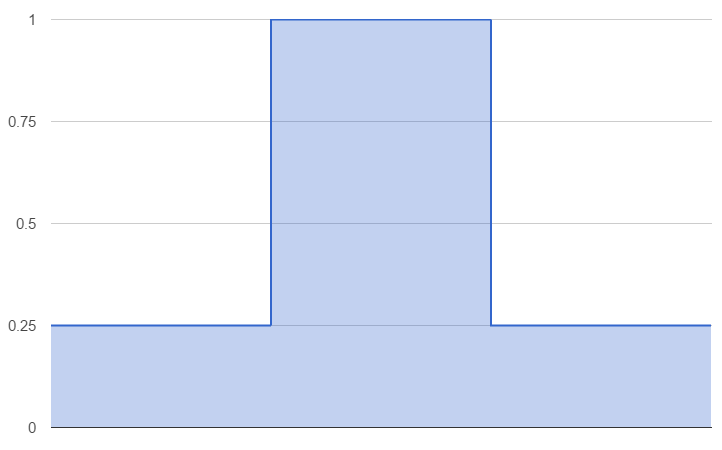
\includegraphics[width=\textwidth]{carga-sintetica1.png}
		\caption{Degrau positivo}
		\label{fig:degrau-positivo}
	\end{subfigure}
	~
	\begin{subfigure}[b]{0.35\textwidth}
		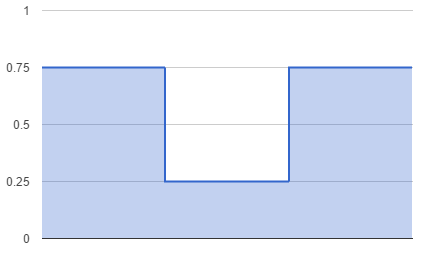
\includegraphics[width=\textwidth]{carga-sintetica2.png}
		\caption{Degrau negativo}
		\label{fig:degrau-negativo}
	\end{subfigure}
	~
	\begin{subfigure}[b]{0.35\textwidth}
		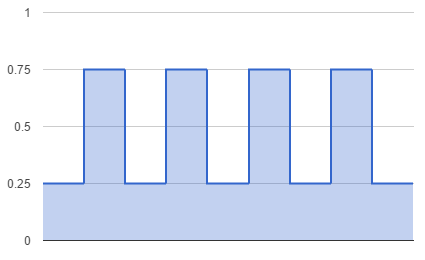
\includegraphics[width=\textwidth]{carga-sintetica3.png}
		\caption{Onda quadrada}
		\label{fig:onda-gradrada}
	\end{subfigure}
	\caption{Possibilidade de cargas moduláveis pela extensão}
	\label{fig:cargas-moduladas-exemplos}
\end{figure}


O Bench4Q simula de um \textit{website} de um \textit{e-commerce}, utilizando uma arquitetura \textit{multi-tier}. Esta arquitetura particiona o processo de aplicação em níveis, onde cada camada fornece uma determinada funcionalidade. Uma vantagem de tal arquitetura é que pode proporcionar um elevado nível de escalabilidade e flexibilidade. No entanto, a alocação de recursos entre esses níveis será mais difícil devido à interdependência entre as camadas. Para a discussão deste trabalho, assumimos um sistema de \textit{multi-tiers} que consiste nos seguintes componentes:

\begin{itemize}
	\item Gerador de Carga (\textit{Workload})
	\item Balanceador de carga (\textit{Load Balancer})
	\item Servidor Físico (\textit{Hypervisor})
	\item Servidor de dados (\textit{Data base})
\end{itemize}


\begin{figure}[!htb]
	\centering
	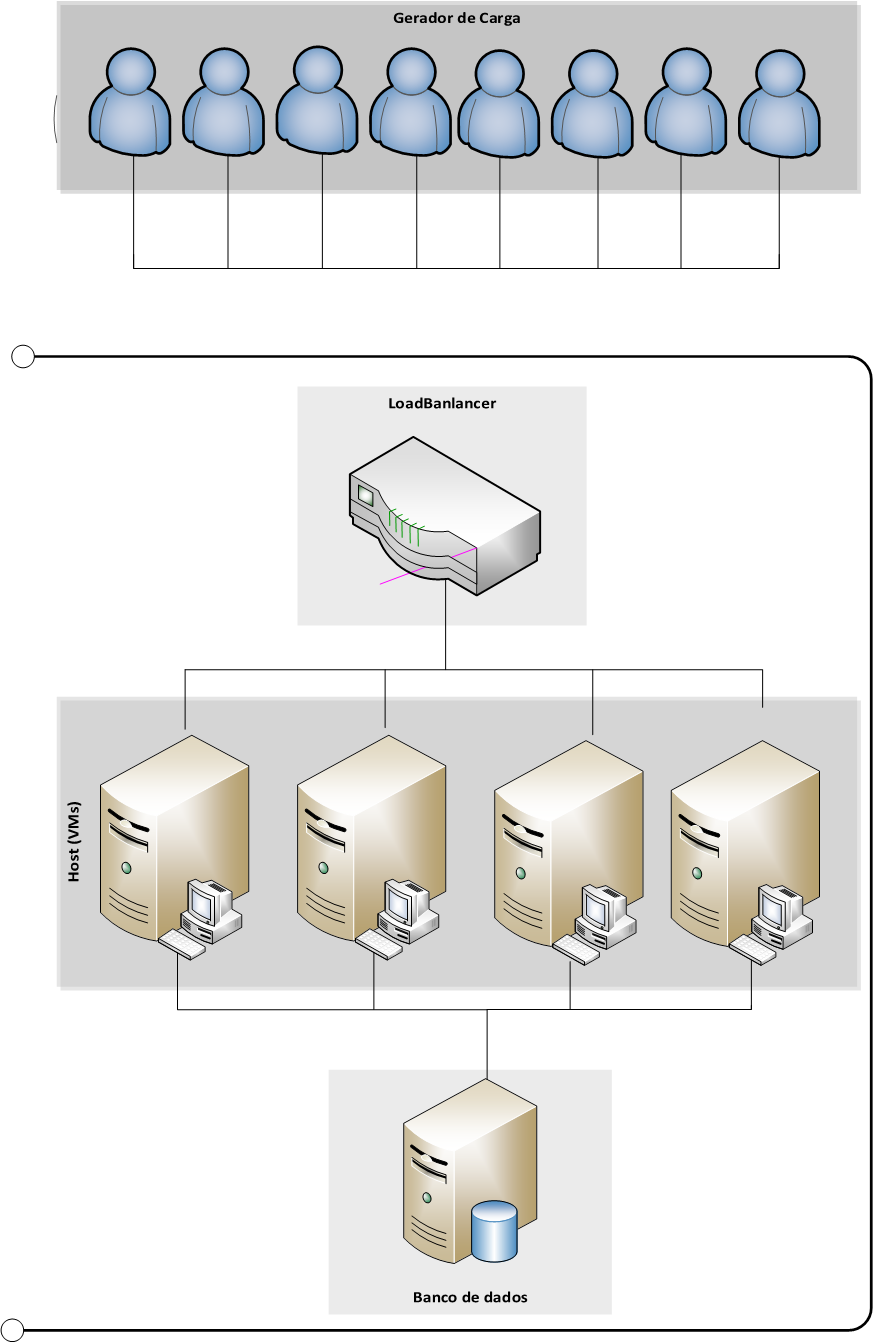
\includegraphics[scale=0.55]{arquitetura-experimento.png}
	\caption{Arquitetura do experimento}
	\label{fig:arquitetura-experimento}
	\fautor
\end{figure}

A arquitetura definida é esquematizado na Figura \ref{fig:arquitetura-experimento}. Os parâmetros do ambiente utilizado para execução dos experimentos são apresentados na Tabela \ref{tab:configuracao_maquinas}.
Foram utilizadas oito unidades para a geração de carga de trabalho (\textit{workload}) que atuam como clientes dos serviços, 1 unidade de balanceamento de carga, 4 servidores atuando como provedor de serviços e 1 unidade executando o banco de dados a ser consultado pelo provedor de serviços.

\begin{table}[htb]
	\centering
	\caption{Especificação do ambiente de execução dos experimentos}
	\label{tab:configuracao_maquinas}
	\begin{tabularx}{\textwidth}{|r|c|X|} \hline\hline
		\textbf{Componente}    & \textbf{Quantidade} & \textbf{Configuração} \\ \hline
		\textit{Workload}      & 8 Unidades          & Intel Core 2 Quad Q9400, 8 GB RAM  \\
		\textit{Load Balancer} & 1 Unidade           & Intel Core I7 3.60GHZ, 32 GB RAM, HD 2TB Sata III \\
		\textit{Hosts}         & 4 Unidades          & Intel Core I7 3.60GHZ, 32 GB RAM, HD 2TB Sata III\\
		\textit{Data base}     & 1 Unidade           & AMD Vishera 4.2 Ghz, 32 GB RAM, HD 2TB Sata III \\
		\hline
	\end{tabularx}
	\fdadospesquisa
\end{table}


%De acordo com \citeonline{KaiSachs2010}, uma metodologia de desenvolvimento de \textit{benchmarks} deve incluir em seu processo de desenvolvimento, bem como a sua execução e a análise dos seus resultados. Para tanto é necessário medir 
O comportamento do sistema é descrito com a base em métricas. A métrica é uma função que transforma resultados medidos em uma forma facilmente compreendida \cite{Folkerts2013}. As métricas de referência devem permitir caracterizar e quantificar o comportamento do sistema quando enfrenta perturbações (ou seja, falhas, ataques, e variações de ambiente operacional) \cite{Marco2012}. As métricas tradicionais, de analise estacionaria, não podem capturar os comportamentos transitórios do sistema em resposta a modulação da carga de trabalho.

%No contexto de avaliação transiente, \citeonline{Rosu1997} afirma que a reatividade da métrica é muitas vezes mais importante do que a otimização da mesma, no mesmo trabalho, 
\citeonline{Rosu1997} apresentam as características e os comportamentos de uma métrica transiente, conforme ilustrado pela Figura \ref{fig:transient-metric}, que são: 
\begin{itemize}
	\item \textbf{\textit{Reaction Time} (Tempo de reação)} - o período entre a ocorrência da variação crítica e a conclusão da promulgação realocação de correção;
	
	\item \textbf{\textit{Recovery Time} (Tempo de Recuperação)} - o intervalo entre a conclusão, promulgação e da restauração de um nível de desempenho aceitável;
	
	\item \textbf{\textit{Performance Laxity} (Frouxidão performance)} - a diferença entre o \textit{required vs performance}, e o desempenho em estado estacionário, após a redistribuição;
\end{itemize}


\begin{figure}[!htb]
	\centering
	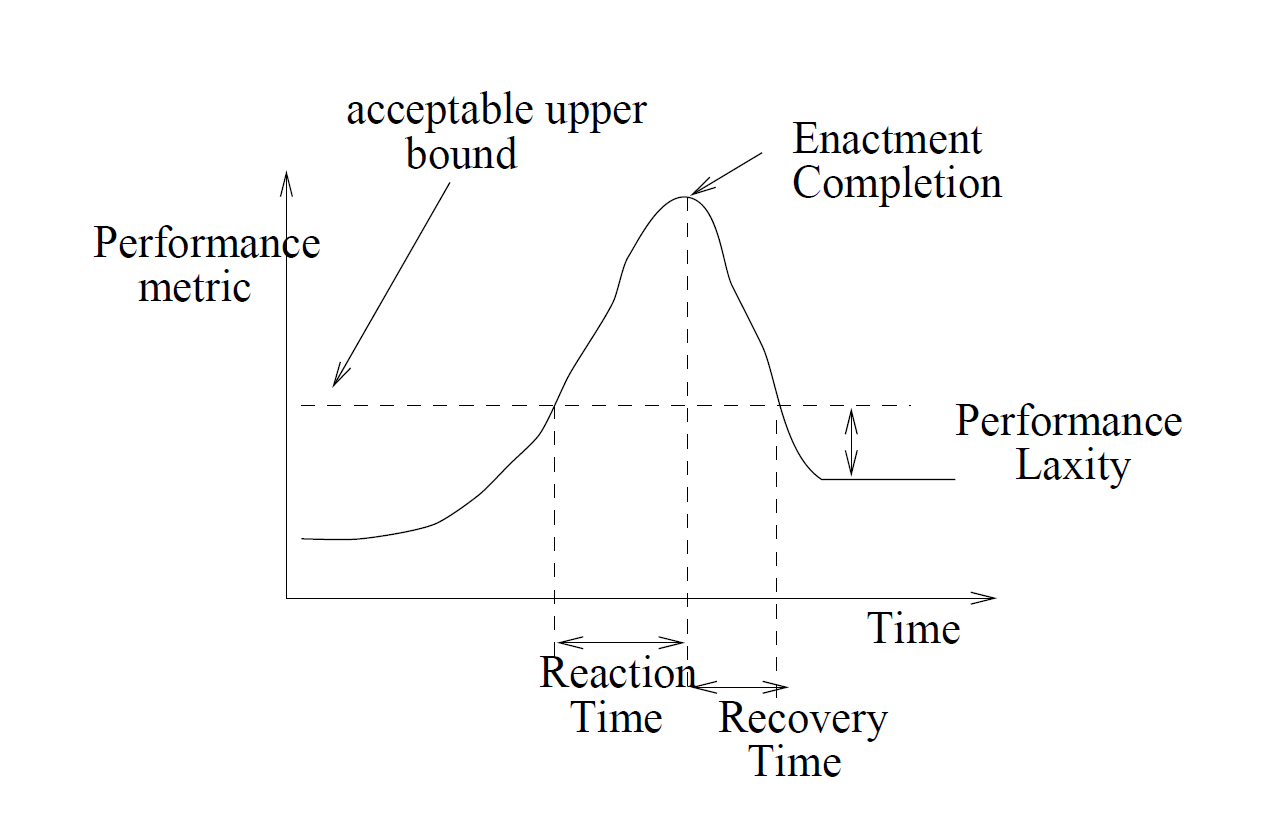
\includegraphics[scale=0.4]{transient-metric.png}
	\caption{Comportamento de métrica transiente}
	\label{fig:transient-metric}
	\fdireta{Rosu1997}		
\end{figure}


A métrica em questão deve ser identificada dentro da realidade e necessidade em que se encontra o sistema a ser avaliado. Logo seria uma ingenuidade fixar um conjunto de métricas para um sistema desconhecido, o importante é que ela tenha o comportamento e as características apresentadas por \citeonline{Rosu1997}. Existem diversos trabalhos dedicados a  identificarem métricas transientes em vários contextos como estado por \citeonline{Binnig2009}, \citeonline{Lu2000} e \citeonline{Rosu1997}.
\citeonline{Binnig2009} afirmam que os \textit{benchmarks} tradicionais estão principalmente preocupados com o desempenho e o custo de sistemas estáticos e essas métricas ainda têm relevância para as aplicações em nuvem, mas é necessário medir diferentes métricas para sistemas escaláveis (ou seja, dinâmicos) onde os recursos vêm e vão. Ainda \citeonline{Binnig2009} enfatiza que os novos \textit{benchmarks} devem relatar métricas diferentes do que os \textit{benchmarks} existentes: 
%\begin{citacao}
	Em vez de medir o desempenho médio de um sistema estático em carga máxima, as novas métricas devem refletir a capacidade dos serviços em nuvem para se adaptar a uma mudança de carga com relação ao desempenho e custos. Além disso, uma métrica adicional também deve cobrir a robustez desses serviços contra falhas de nós individuais.
%\end{citacao}

As métricas definidas precisam refletir o cenário de dinâmica do sistema, é interessante também cobrir cada um dos níveis da arquitetura proposta. Neste projeto é interessante salientar:
\begin{itemize}
	\item \textbf{Conexões por segundo (\textit{Load Balancer}):} Conforme sugerido por \citeonline{Binnig2009}, medir a escalabilidade através do aumento dos interações web emitidos por segundo ao longo do tempo e de forma contínua contando a interação web que são respondidas em um intervalo de tempo de resposta,
	
	\item \textbf{Tempo de resposta (\textit{browsers}):} \citeonline{helder2014}, em um sistema dinâmico, cuja transformação entrada-saída não ocorre em tempo zero, mas é sujeita a uma inércia advinda dos processos físicos associados, possuí uma inércia intrínseca que atrasa o efeito que uma entrada terá na saída. Esses efeitos refletem no consequentemente nos comportamentos diversos que incluem retardo no tempo de resposta e possíveis oscilações; 
	
	\item \textbf{Taxa de utilização da CPU (VMs):} \citeonline{Nobile2013} afirma que diversas métricas podem ser analisadas para verificar o desempenho das máquinas virtuais, e cita alguns exemplos, como o tempo de inicialização, a taxa de utilização de CPU, o tempo médio de resposta e o \textit{throughput}, e usualmente, número de máquinas virtuais que hospedam serviços de interesse ao cliente e que respondem a uma carga de trabalho imposta por usuários através de requisições;

	\item \textbf{Taxa de utilização da CPU:} O trabalho apresentado por \citeonline{wang2009}, que lida com uma carga de trabalho variante no tempo e intensiva, demonstra que a CPU e I/O podem ser utilizadas para prever as necessidades dos recursos de um banco de dados e para orientar a alocação de recursos \textit{on-demand} de acordo com a exigência de carga de trabalho. Entretanto iremos somente considerar em nossos experimento a taxa de utilização do banco de dados.
\end{itemize}


Uma vez que a extensão é desenvolvida e a configuração física do ambiente é estabelecida, a configuração lógica do ambiente de medição tem de ser especificada. Nesse contexto, é de interesse analisar o impacto da carga de trabalho no ambiente. Logo, se faz necessário efetuar um experimento com uma carga de trabalho modelada, bem como a formulação subsequente do experimento. 
%O principal objeto de estudo dessa analise, tem por objeto o impacto de uma carga de trabalho modela pela extensão feita no \textit{benchmark} no ambiente.

Considerando a utilização de um ambiente físico real e controlado juntamente com o objetivo experimental, utilizamos um único fator, a carga de trabalho (\textit{workload}) conforme apresentado na Tabela \ref{tab:fatores_niveis}.
\begin{table}[htb]
	\centering
	\caption{Fator e nível dos experimentos}
	\label{tab:fatores_niveis}
	\begin{tabularx}{\textwidth}{|r|X|} \hline\hline
		\textbf{Fator}		& \textbf{\textit{Workload}} \\ \hline
		\textit{Nível 1}	&		20 EBs				 \\
		\textit{Nível 2}	&		60 EBs				 \\		
		\hline
	\end{tabularx}
	\fdadospesquisa
\end{table}

O único fator refere-se à quantidade de clientes simultâneos requisitando o serviço do \textit{e-commerce}. Esses clientes são modulados conforme a configuração feita. São feitas assim essa carga de trabalho estimulará o sistema a apresentar a sua dinâmica. Neste estudo, 3 replicações para cada experimento.
Durante a execução dos experimentos, pequenas aplicações, monitores, em cada um dos níveis da arquitetura são responsáveis por coletar algumas informações de interesse disponíveis, como a taxa de utilização de CPU e a quantidade de requisições simultâneas. Os valores produzidos pela experimentação foram adicionados em arquivos Excel (\textit{.xls}) e processados pelo R \footnote{\url{https://www.r-project.org/}}.
